\documentclass[conference]{IEEEtran}
\usepackage[utf8]{inputenc}
\usepackage[T1]{fontenc}
\usepackage[spanish,es-tabla,es-nodecimaldot]{babel}
\usepackage{graphicx}
\usepackage{url}
\usepackage{amsmath}

\renewcommand{\IEEEkeywordsname}{Palabras clave}
% Autores: reemplazar "Autor 1, Autor 2..." y los correos por los datos reales.
\begin{document}

\title{Sistema inteligente de análisis de PQRS con data lake, harness y un modelo de lenguaje local}

\author{
\IEEEauthorblockN{Autor 1, Autor 2, Autor 3}
\IEEEauthorblockA{Programa de Ingeniería de Sistemas\\
Corporación Universitaria Minuto de Dios -- UNIMINUTO\\
Bogotá, Colombia\\
correo1@uniminuto.edu.co, correo2@uniminuto.edu.co}
}

\maketitle

\begin{abstract}
Las universidades reciben peticiones, quejas, reclamos y sugerencias (PQRS) por canales de formatos mezclados: texto, audio y fotografías de formularios. Su revisión manual retrasa las respuestas y oculta los casos urgentes. Este artículo presenta la arquitectura y la implementación de un sistema que almacena las PQRS sin transformar en un data lake compatible con S3, las convierte en texto dentro de un harness contenerizado (Whisper para audio y Tesseract para imágenes) y las clasifica por tipo, tema y urgencia con un modelo de lenguaje de 3.000 millones de parámetros que corre localmente, sin servicios en la nube. Una aplicación web adaptable a celulares permite radicar PQRS con varias partes, seguir su estado y gestionarlas por área. Sobre 30 casos sintéticos, la versión final alcanzó 86,7\,\% de precisión en tipo y tema, 73,3\,\% en urgencia y detectó 7 de 8 casos de urgencia alta. Se discuten las prácticas de desarrollo, la reproducibilidad entre equipos y las limitaciones del estudio.
\end{abstract}

\begin{IEEEkeywords}
PQRS, data lake, harness, modelos de lenguaje, clasificación de texto, arquitectura de software, Docker.
\end{IEEEkeywords}

\section{Introducción}
El derecho de petición obliga a las instituciones colombianas a responder las solicitudes de los ciudadanos en plazos definidos; la Ley 1755 de 2015 fija como regla general un término de quince días hábiles \cite{ley1755}. En una universidad, las PQRS llegan por correo, formularios web, llamadas y formularios en papel, y su revisión suele ser manual. Esto produce tres problemas: respuestas tardías, casos urgentes que pasan desapercibidos y poca información agregada para las directivas.

El objetivo de este trabajo fue diseñar e implementar un prototipo que reciba PQRS en cualquier formato, las clasifique automáticamente y las enrute al área responsable, conservando los datos en el equipo de la institución. Las PQRS contienen datos personales, cuya protección regula la Ley 1581 de 2012 \cite{ley1581}; por eso se usó un modelo de lenguaje local en lugar de un servicio externo.

Los aportes son: (i) una arquitectura que separa el almacenamiento de originales (data lake), el procesamiento (harness) y los datos estructurados (base de datos); (ii) un flujo que admite PQRS con texto, audio y fotografía en un mismo caso; (iii) una evaluación iterativa del clasificador con datos sintéticos etiquetados, y (iv) una discusión de las prácticas de desarrollo y de la reproducibilidad del sistema.

\section{Marco normativo y conceptual}
\subsection{Normas de referencia}
La descripción de la arquitectura sigue la noción de vistas y preocupaciones de la norma ISO/IEC/IEEE 42010 \cite{iso42010}: se presentan una vista lógica (componentes y flujo) y una vista de despliegue. Los procesos de desarrollo se organizaron con referencia a ISO/IEC/IEEE 12207 \cite{iso12207} (requisitos, diseño, construcción, pruebas) y los atributos de calidad se analizan con el modelo de ISO/IEC 25010 \cite{iso25010}.

\subsection{Data lake}
Un data lake almacena datos en su formato original, sin imponer una estructura previa, a diferencia de una bodega de datos \cite{dixon}. Esto lo hace adecuado para PQRS que llegan como audio, imagen o texto: el original se conserva intacto y el procesamiento produce, aparte, datos estructurados.

\subsection{Harness y contenedores}
En este trabajo, el harness es el entorno controlado donde se ejecuta el procesamiento: un contenedor con las herramientas instaladas, que lee del data lake sin modificar los originales, ejecuta las tareas en orden y deja el resultado en la base de datos. Los contenedores \cite{docker} permiten que el mismo entorno se reproduzca en cualquier equipo con Docker.

\subsection{Extracción de texto y modelos de lenguaje}
Whisper es un modelo de reconocimiento de voz entrenado con supervisión débil a gran escala \cite{whisper}; Tesseract es un motor de reconocimiento óptico de caracteres de código abierto \cite{tesseract}. Para la clasificación se usó Llama 3.2 en su versión de 3.000 millones de parámetros, de la familia Llama 3 \cite{llama3}, servido localmente con Ollama \cite{ollama}. La instrucción al modelo incluye ejemplos resueltos (aprendizaje con pocos ejemplos) \cite{brown} y le pide una justificación breve antes de decidir la urgencia, una forma acotada de razonamiento paso a paso \cite{cot}.

\section{Arquitectura}
\begin{figure*}[!t]
\centering
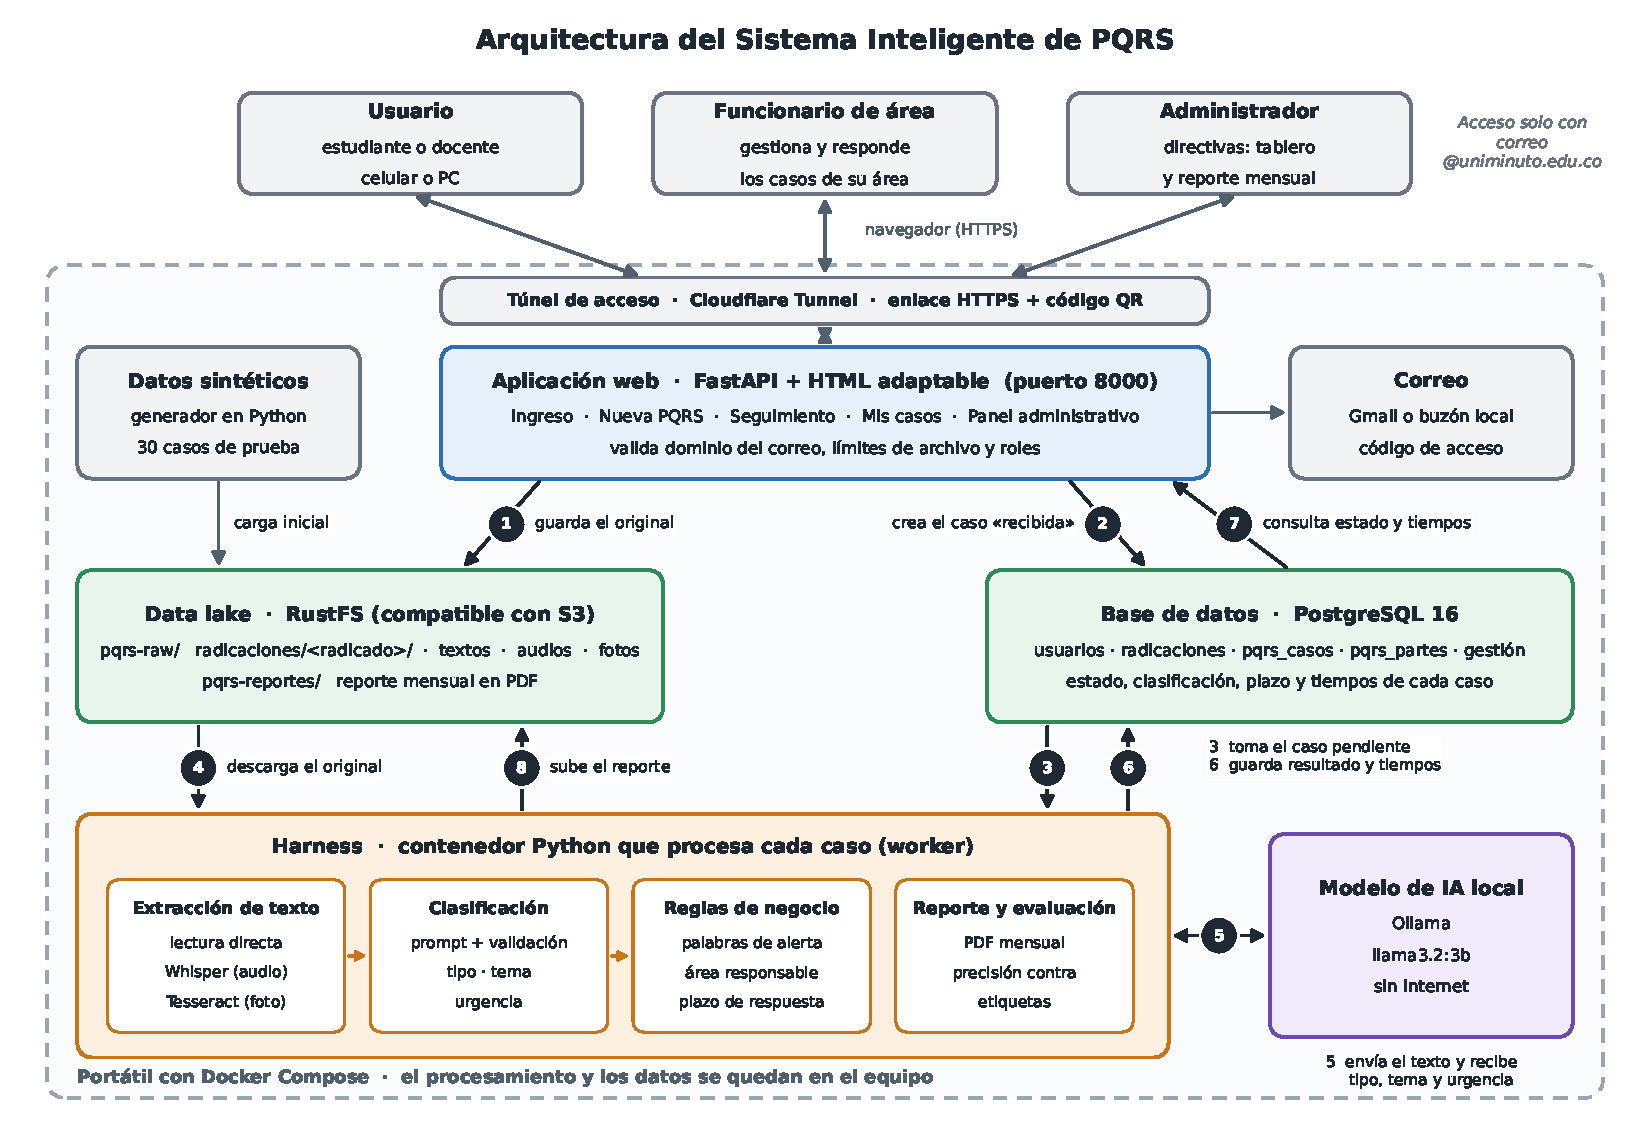
\includegraphics[width=0.86\textwidth]{arquitectura_pqrs.pdf}
\caption{Vista lógica: componentes y flujo de un caso (pasos 1 a 8).}
\label{fig:arquitectura}
\end{figure*}

La Fig.~\ref{fig:arquitectura} muestra la vista lógica. Todos los componentes corren como contenedores de Docker Compose en un mismo equipo:
\begin{itemize}
\item \textbf{Aplicación web} (FastAPI): ingreso, radicación, seguimiento y panel de gestión.
\item \textbf{Data lake} (RustFS, compatible con S3): originales y reportes.
\item \textbf{Base de datos} (PostgreSQL 16): casos, partes, usuarios, gestión e historial.
\item \textbf{Harness} (Python 3.11): extracción, clasificación, reporte y evaluación; en producción corre como un proceso que revisa el data lake cada 3~s.
\item \textbf{Modelo local} (Ollama con \texttt{llama3.2:3b}).
\end{itemize}

\subsection{Flujo de un caso}
El usuario radica la PQRS en la web. Cada parte (texto, audio o foto) se guarda en una carpeta propia del data lake y, al final, se escribe un \emph{manifiesto} con la lista de partes. El harness solo procesa una carpeta cuando encuentra su manifiesto, lo que evita tomar paquetes incompletos. Luego extrae el texto de cada parte, los une con etiquetas en un orden fijo (texto escrito, transcripción, texto de la foto) y clasifica el caso una sola vez. El resultado y el tiempo de cada etapa se guardan en la base de datos, y la web los muestra al usuario.

\subsection{Decisiones de diseño}
\textit{Separación entre la IA y las reglas.} El modelo solo decide tipo, tema y urgencia dentro de catálogos cerrados. El área responsable se deriva del tema con una tabla fija, y una regla eleva a urgencia alta los mensajes con vocabulario de riesgo (acoso, amenaza, emergencia, entre otros). Así, los casos críticos no dependen únicamente del modelo.

\textit{Trazabilidad.} La corrección de un funcionario se guarda aparte de la respuesta del modelo, lo que permite auditar y medir cuánto se equivoca el sistema en uso real.

\textit{Independencia del proveedor.} El acceso al almacenamiento usa el protocolo S3. El plan inicial era MinIO, pero sus imágenes públicas dejaron de estar disponibles durante el proyecto; el cambio a RustFS solo requirió modificar la configuración del contenedor.

\textit{Intercambiabilidad del modelo.} El clasificador es un módulo con una sola función de entrada; una variable de entorno permite cambiar el modelo local por uno en la nube sin tocar el resto del sistema.

\subsection{Vista de despliegue}
\begin{figure*}[!t]
\centering
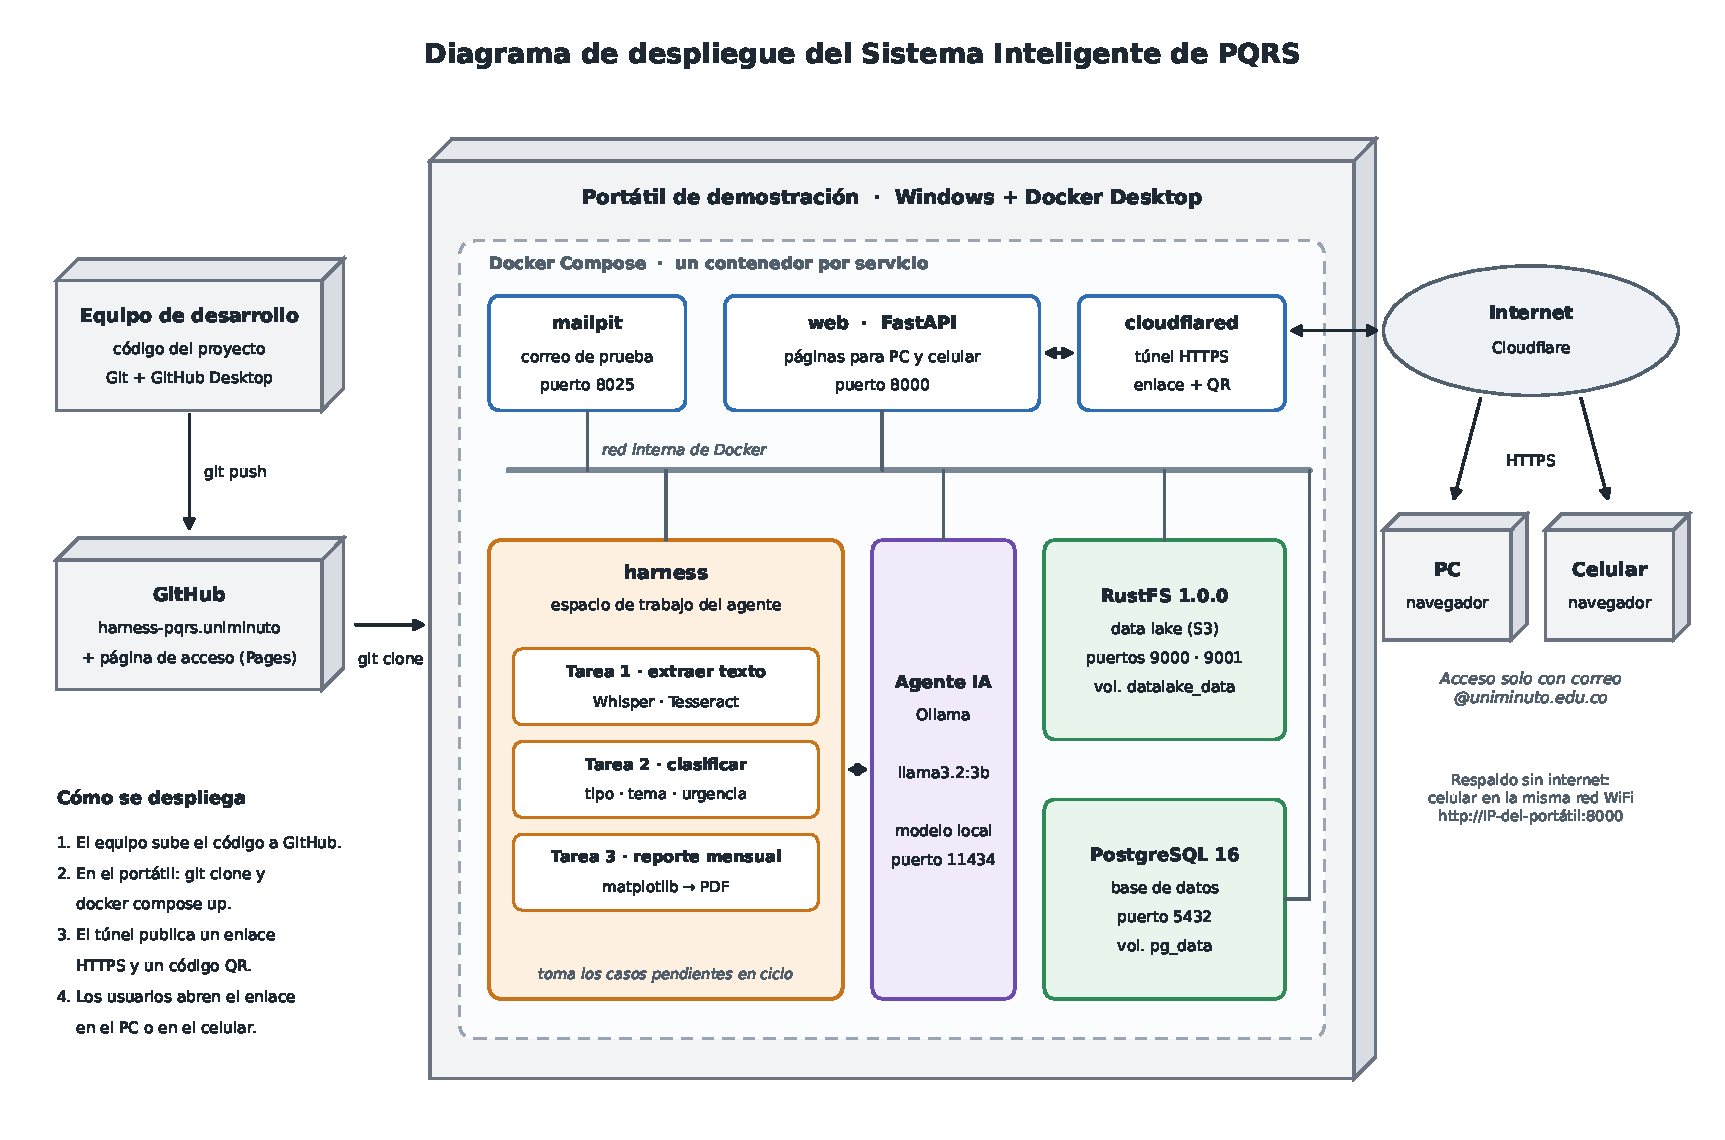
\includegraphics[width=0.78\textwidth]{despliegue_pqrs.pdf}
\caption{Vista de despliegue.}
\label{fig:despliegue}
\end{figure*}

La Fig.~\ref{fig:despliegue} muestra el despliegue. El código está en GitHub y un portátil con Docker ejecuta todos los servicios. Para el acceso desde otros dispositivos, un túnel HTTPS publica un enlace temporal, y una página estática en GitHub Pages redirige siempre al enlace vigente. El procesamiento y los datos permanecen en el equipo; el túnel solo transporta la conexión cifrada del navegador.

\section{Implementación y prácticas de desarrollo}
\subsection{Datos sintéticos}
No se usaron PQRS reales. Un generador con semilla fija produce 30 casos (10 textos, 10 audios con voz sintética y 10 imágenes de formularios), con su clasificación correcta en un archivo de etiquetas. La semilla garantiza que cualquier equipo genere exactamente los mismos casos.

\subsection{Desarrollo iterativo del clasificador}
El clasificador se mejoró en tres versiones, midiendo cada una contra las etiquetas: v1, con una instrucción básica; v2, con criterios explícitos para cada categoría, seis ejemplos distintos a los casos de prueba y un campo de justificación de la urgencia; y v3, que añade la regla de vocabulario de riesgo. El modelo se consulta con temperatura cero y salida obligatoria en JSON; las respuestas fuera de catálogo se registran en lugar de ocultarse.

\subsection{Pruebas}
Además de la evaluación del clasificador, se probaron las reglas de la aplicación (dominio institucional del correo, límites de archivos, roles por área y transiciones de estado), un caso con texto, audio y foto de extremo a extremo, y la instalación desde cero clonando el repositorio y siguiendo solo su documentación.

\subsection{Uso de asistentes de IA}
El desarrollo contó con un asistente de IA para generar y revisar código. Las decisiones de diseño, las pruebas y la interpretación de los resultados fueron verificadas por el equipo. La sección final del artículo declara este uso.

\section{Resultados}
\begin{table}[!t]
\caption{Precisión del clasificador sobre 30 casos sintéticos}
\label{tab:resultados}
\centering
\begin{tabular}{lccc}
\hline
\textbf{Medida} & \textbf{v1} & \textbf{v2} & \textbf{v3} \\
\hline
Tipo & 80,0\,\% & 86,7\,\% & 86,7\,\% \\
Tema & 86,7\,\% & 86,7\,\% & 86,7\,\% \\
Urgencia & 56,7\,\% & 66,7\,\% & 73,3\,\% \\
Los tres campos & 40,0\,\% & 46,7\,\% & 50,0\,\% \\
Urgencias altas detectadas & 87,5\,\% & 62,5\,\% & 87,5\,\% \\
\hline
\end{tabular}
\end{table}

La Tabla~\ref{tab:resultados} resume la evaluación. La v2 mejoró el tipo y la urgencia, pero dejó de detectar tres casos de urgencia alta, entre ellos un mensaje de malestar emocional clasificado como urgencia baja. La regla de vocabulario de riesgo (v3) recuperó esos casos y llevó la urgencia a 73,3\,\%. Los errores de tipo se concentraron en un patrón: el modelo tiende a clasificar como petición mensajes que eran quejas, reclamos o sugerencias.

\textit{Reproducibilidad.} La misma configuración, ejecutada en un segundo equipo, obtuvo los mismos valores salvo en el tema (83,3\,\%), por un único caso distinto. Se verificó que la instrucción enviada al modelo era idéntica en ambos equipos; la diferencia se atribuyó a la versión del servidor del modelo, que no estaba fijada. A partir de este hallazgo, la versión de Ollama quedó fijada en la configuración.

\textit{Caso de varias partes.} En una PQRS con texto, audio y fotografía, la transcripción del audio (7,5~s) y el texto de la fotografía (0,5~s) coincidieron palabra por palabra con los originales. La primera clasificación tardó alrededor de 80~s, porque el modelo se carga en memoria; las siguientes tardaron alrededor de 19~s en un portátil sin GPU.

\textit{Atributos de calidad.} En términos de ISO/IEC 25010 \cite{iso25010}, el diseño favorece la \emph{seguridad} (datos locales, acceso solo con correo institucional y códigos de un solo uso), la \emph{mantenibilidad} (módulos intercambiables y reglas separadas del modelo) y la \emph{portabilidad} (contenedores y documentación de instalación). La \emph{eficiencia de desempeño} es su punto débil: la clasificación en CPU tarda decenas de segundos por caso.

\section{Limitaciones y trabajo futuro}
Los 30 casos son sintéticos y la instrucción y las reglas se ajustaron observando esos mismos casos; no hubo un conjunto de prueba independiente, por lo que los porcentajes son optimistas e indicativos. Las etiquetas correctas las definió el equipo, y la frontera entre urgencia media y alta es subjetiva. Las PQRS de varias partes funcionan, pero no se evaluaron con un conjunto propio. Cuando el modelo responde un valor fuera de catálogo, el sistema usa un valor por defecto en lugar de enviar el caso a revisión manual. Como trabajo futuro se propone: un conjunto de prueba independiente validado por varias personas, la evaluación de casos de varias partes, la comparación con modelos más grandes y la ejecución en un servidor institucional.

\section{Conclusiones}
Es viable clasificar PQRS de formatos mezclados con herramientas libres que corren en un solo equipo, sin enviar datos personales a terceros. La separación entre data lake, harness y base de datos permitió agregar nuevos canales, como las PQRS con varias partes, sin rehacer el procesamiento. El modelo de 3.000 millones de parámetros es suficiente para el tipo y el tema, pero no es confiable por sí solo para la urgencia: combinarlo con reglas explícitas y con la revisión de un funcionario fue la decisión que más aportó a la seguridad del sistema. Fijar versiones y generar los datos con una semilla resultó indispensable para que los resultados se puedan repetir.

\section*{Declaración de uso de inteligencia artificial}
En la elaboración del código y de este artículo se usó un asistente de inteligencia artificial (Claude, de Anthropic) para generar y revisar código, documentación y redacción. El equipo verificó el funcionamiento del sistema, los resultados reportados y el contenido del texto, y asume la responsabilidad por ellos.

\begin{thebibliography}{99}
\bibitem{ley1755} Congreso de Colombia, ``Ley 1755 de 2015, por medio de la cual se regula el derecho fundamental de petición,'' \emph{Diario Oficial}, 30 jun. 2015.
\bibitem{ley1581} Congreso de Colombia, ``Ley Estatutaria 1581 de 2012, por la cual se dictan disposiciones generales para la protección de datos personales,'' \emph{Diario Oficial}, 18 oct. 2012.
\bibitem{iso42010} \emph{Software, systems and enterprise --- Architecture description}, ISO/IEC/IEEE 42010:2022, 2022.
\bibitem{iso12207} \emph{Systems and software engineering --- Software life cycle processes}, ISO/IEC/IEEE 12207:2017, 2017.
\bibitem{iso25010} \emph{Systems and software engineering --- Systems and software Quality Requirements and Evaluation (SQuaRE) --- Product quality model}, ISO/IEC 25010:2023, 2023.
\bibitem{dixon} J. Dixon, ``Pentaho, Hadoop, and data lakes,'' blog de James Dixon, oct. 2010.
\bibitem{docker} D. Merkel, ``Docker: Lightweight Linux containers for consistent development and deployment,'' \emph{Linux Journal}, vol. 2014, no. 239, 2014.
\bibitem{whisper} A. Radford, J. W. Kim, T. Xu, G. Brockman, C. McLeavey e I. Sutskever, ``Robust speech recognition via large-scale weak supervision,'' en \emph{Proc. 40th Int. Conf. Machine Learning (ICML)}, 2023, pp. 28492--28518.
\bibitem{tesseract} R. Smith, ``An overview of the Tesseract OCR engine,'' en \emph{Proc. 9th Int. Conf. Document Analysis and Recognition (ICDAR)}, 2007, pp. 629--633.
\bibitem{llama3} A. Grattafiori \emph{et al.}, ``The Llama 3 herd of models,'' arXiv:2407.21783, 2024.
\bibitem{ollama} Ollama, ``Ollama,'' 2026. [En línea]. Disponible: \url{https://ollama.com}
\bibitem{brown} T. B. Brown \emph{et al.}, ``Language models are few-shot learners,'' en \emph{Advances in Neural Information Processing Systems}, vol. 33, 2020, pp. 1877--1901.
\bibitem{cot} J. Wei \emph{et al.}, ``Chain-of-thought prompting elicits reasoning in large language models,'' en \emph{Advances in Neural Information Processing Systems}, vol. 35, 2022, pp. 24824--24837.
\end{thebibliography}

\end{document}
